% Required packages:
% \usepackage{booktabs}
% \usepackage{graphicx}
% \usepackage{multirow}

\section{Results}

We evaluate rolling ICU surveillance under two interfaces. In the autoformalized \texttt{session\_tools} setting, the agent interacts with a structured function and guideline layer. In the \texttt{zeroshot\_python} setting, the agent reasons directly over checkpoint-scoped raw MIMIC-IV tables through Python and \texttt{query\_db}. Across both settings, the model must output a structured surveillance state, including \texttt{suspected\_conditions} and \texttt{alerts}, while \texttt{global\_action} and \texttt{priority} serve only as compressed response-layer summaries.

\subsection{Results Summary / Introduction}

Our primary benchmark is the autoformalized \texttt{benchmark\_2k} evaluation, which contains 2{,}000 ICU stays and 26{,}000 checkpoint decisions. On this benchmark, the strongest fully completed model is \texttt{Qwen3.5-27B}, which achieves the best completed-run \texttt{suspected\_conditions\_macro\_f1} (0.1472) and misses fewer alerting trajectories (909) than the smaller completed Qwen variants. However, even the best completed model remains far from reliable longitudinal surveillance: \texttt{alerts\_macro\_f1} remains near 0.24, exact set recovery remains low, and strict patient-level exactness is only 1.10\%. A partial \texttt{gpt-oss-120b} run is stronger on several metrics, but because it completed only 1{,}026/2{,}000 trajectories, it should be treated as provisional.

The zero-shot raw-table setting produces a different short-pilot ranking on \texttt{benchmark\_100}. Here the closed-source models are substantially stronger than the open-weight models. \texttt{Gemini 3.1 Pro Preview} achieves the best suspect-family recovery (0.4393 macro F1), while \texttt{Claude Sonnet 4.6} achieves the best alert-family recovery (0.4722 macro F1) and first-alert timing (3.95h mean absolute error). However, there is no completed zero-shot \texttt{benchmark\_2k} comparison, so these results should be interpreted as backend-specific pilot evidence rather than as a replacement for the main benchmark.

\begin{table*}[t]
\centering
\caption{Primary autoformalized \texttt{benchmark\_2k} results. This is the main benchmark table because it evaluates the full 2{,}000-stay rolling surveillance task and directly scores structured disease-family recovery plus patient-level temporal quality.}
\label{tab:surv_main_benchmark2k}
\resizebox{\textwidth}{!}{%
\begin{tabular}{lrrrrrrrrrrr}
\toprule
Model & Completed stays & Suspect F1 & Alert F1 & Alert Prec. & Alert Recall & Suspect Exact & Alert Exact & First-alert MAE (h) & False-early & Missed alerts & Strict traj. exact \\
\midrule
\texttt{Qwen3.5-27B} & 2000/2000 & 0.1472 & 0.2423 & 0.2643 & 0.2355 & 0.1239 & 0.2195 & 10.6119 & 37 & 909 & 0.0110 \\
\texttt{Qwen3.5-4B}  & 2000/2000 & 0.1396 & 0.2453 & 0.2647 & 0.2390 & 0.1171 & 0.2232 & 9.5982  & 34 & 982 & 0.0090 \\
\texttt{Qwen3.5-9B}  & 2000/2000 & 0.1366 & 0.2456 & 0.2707 & 0.2380 & 0.1266 & 0.2213 & 12.1627 & 17 & 998 & 0.0115 \\
\texttt{gpt-oss-120b} & 1026/2000 & 0.2054 & 0.2533 & 0.2759 & 0.2476 & 0.1276 & 0.2123 & 6.8496  & 58 & 209 & 0.0049 \\
\texttt{gemma-4-31B-it} & 1714/2000 & 0.1344 & 0.2277 & 0.2304 & 0.2269 & 0.1309 & 0.2253 & 22.9554 & 2 & 1455 & 0.0117 \\
\bottomrule
\end{tabular}%
}
\end{table*}

\subsection{Longitudinal State Tracking Is the Core Bottleneck}

The central empirical result is that coarse checkpoint plausibility does not translate into correct longitudinal state tracking. Models often recover enough local evidence to choose a reasonable top-level surveillance posture, but they fail to maintain the correct evolving disease-family state over time. This is visible in three ways.

First, family-level structured-state metrics remain much lower than coarse summary metrics. For example, on autoformalized \texttt{benchmark\_2k}, \texttt{Qwen3.5-27B} reaches 0.4577 \texttt{global\_action\_accuracy}, yet only 0.1472 \texttt{suspected\_conditions\_macro\_f1}. The benchmark therefore cannot be characterized as a simple escalation-versus-monitoring task; the harder problem is reconstructing the correct family-state configuration behind the action.

Second, patient-level alerting remains brittle. Even when a model eventually emits some correct signals, it frequently misses entire alerting trajectories. On \texttt{benchmark\_2k}, the completed Qwen runs miss 909, 998, and 982 alerting stays respectively. This indicates that the dominant failure is not minor timing noise, but failure to carry the appropriate surveillance state forward across the stay.

Third, strict longitudinal exactness remains near zero. Requiring exact agreement on \texttt{global\_action}, \texttt{priority}, \texttt{suspected\_conditions}, and \texttt{alerts} at every checkpoint yields only 0.90\% to 1.15\% accuracy for the completed autoformalized Qwen runs. This harsh metric is nonetheless appropriate for a rolling surveillance benchmark: the clinical burden lies in sustaining coherent state over time, not merely in producing isolated locally plausible answers.

The same conclusion becomes sharper when suspect and alert metrics are decomposed into overall, negative-set, and positive-set checkpoints. Overall \texttt{alerts\_exact\_match} clusters near 0.22, but this is largely driven by negative-set checkpoints where the gold alert set is empty. On the completed Qwen \texttt{benchmark\_2k} runs, negative-only \texttt{alert\_exact} is 0.9477--0.9647, whereas positive-only \texttt{alert\_exact} is only 0.0038--0.0112. Positive-only \texttt{alert\_macro\_f1} remains only 0.0343, 0.0352, and 0.0398. Thus, the benchmark's real difficulty lies in recovering active structured state, not in preserving emptiness.

\begin{table*}[t]
\centering
\caption{Decomposition of the completed Qwen \texttt{benchmark\_2k} runs into overall, negative-set, and positive-set checkpoints. The clustering of overall exact-match metrics is largely a negative-set effect; positive-set recovery remains extremely weak.}
\label{tab:surv_decomp_qwen2k}
\resizebox{\textwidth}{!}{%
\begin{tabular}{llrrrrrr}
\toprule
Model & Slice & Suspect Exact & Suspect F1 & Alert Exact & Alert F1 & Alert Prec. & Alert Recall \\
\midrule
\texttt{Qwen3.5-27B} & overall        & 0.1239 & 0.1472 & 0.2195 & 0.2423 & 0.2643 & 0.2355 \\
\texttt{Qwen3.5-27B} & negative only  & 0.9189 & 0.9189 & 0.9529 & 0.9529 & 0.9529 & 0.9529 \\
\texttt{Qwen3.5-27B} & positive only  & 0.0071 & 0.0338 & 0.0049 & 0.0343 & 0.0628 & 0.0255 \\
\texttt{Qwen3.5-9B}  & overall        & 0.1266 & 0.1366 & 0.2213 & 0.2456 & 0.2707 & 0.2380 \\
\texttt{Qwen3.5-9B}  & negative only  & 0.9601 & 0.9601 & 0.9647 & 0.9647 & 0.9647 & 0.9647 \\
\texttt{Qwen3.5-9B}  & positive only  & 0.0041 & 0.0156 & 0.0038 & 0.0352 & 0.0676 & 0.0253 \\
\texttt{Qwen3.5-4B}  & overall        & 0.1171 & 0.1396 & 0.2232 & 0.2453 & 0.2647 & 0.2390 \\
\texttt{Qwen3.5-4B}  & negative only  & 0.8766 & 0.8766 & 0.9477 & 0.9477 & 0.9477 & 0.9477 \\
\texttt{Qwen3.5-4B}  & positive only  & 0.0055 & 0.0313 & 0.0112 & 0.0398 & 0.0648 & 0.0317 \\
\bottomrule
\end{tabular}%
}
\end{table*}

The temporal-semantic analysis points to the same bottleneck. In the completed Qwen \texttt{benchmark\_2k} runs, performance is consistently strongest on \texttt{active\_interval} states, weaker on \texttt{recent\_measurement + TTL}, and extremely poor on \texttt{persistent\_episode}, \texttt{cumulative\_max\_stage}, and \texttt{composite\_current\_state}. This means the models can partially identify currently visible support states, but rarely maintain persistent sepsis-related state, preserve cumulative AKI stage, or recompute composite shock states correctly.

\begin{figure*}[t]
\centering
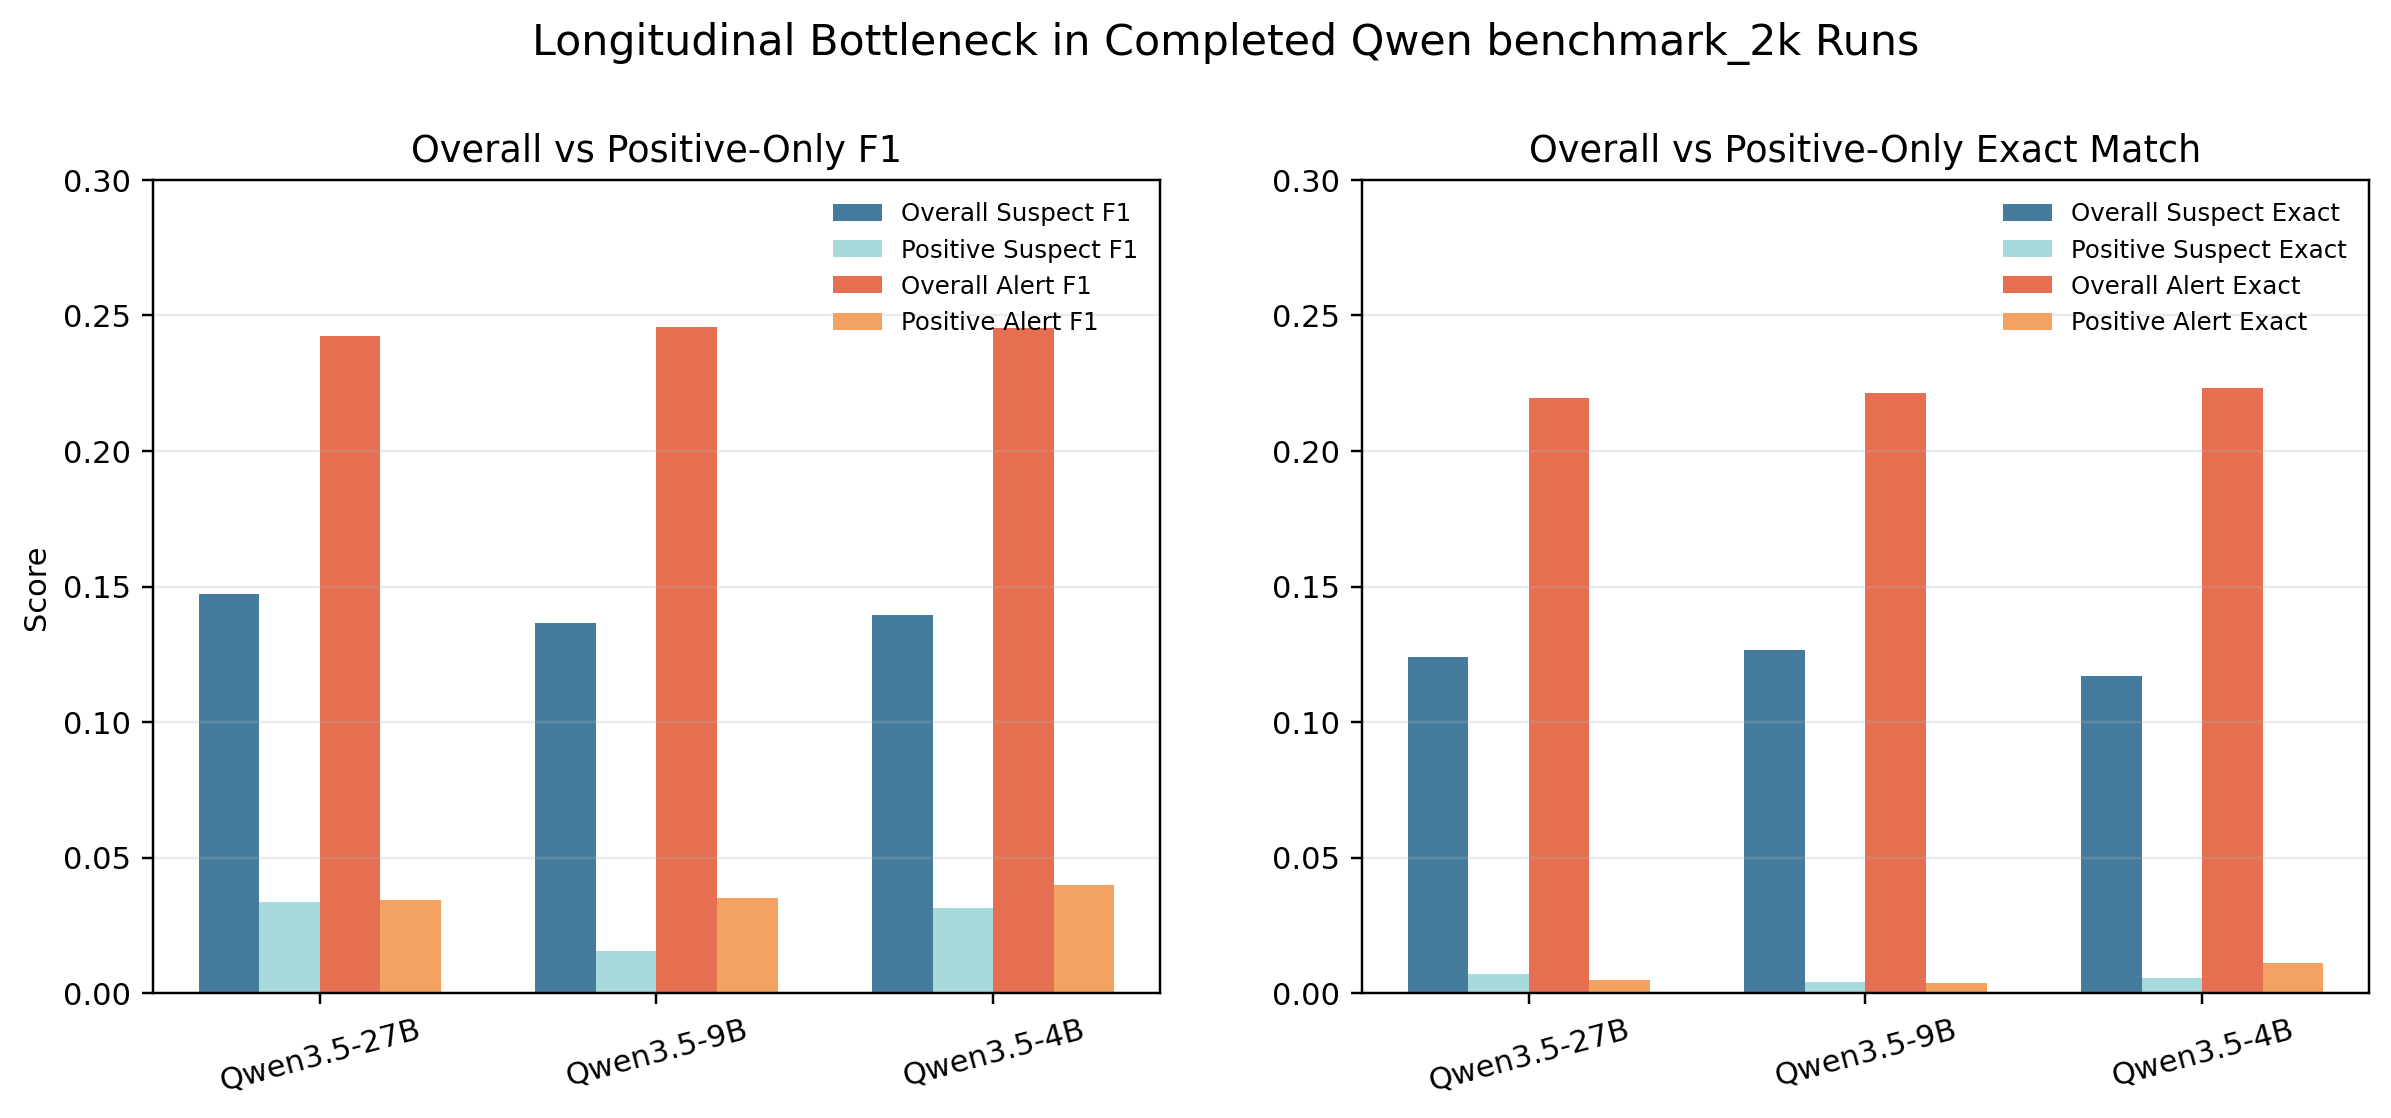
\includegraphics[width=0.78\textwidth]{figures/qwen_benchmark2k_bottleneck_decomposition.png}
\caption{Overall versus positive-only structured-state metrics for the completed Qwen \texttt{benchmark\_2k} runs. The apparent moderate overall scores collapse once evaluation is restricted to positive suspect and alert checkpoints.}
\label{fig:qwen_bottleneck}
\end{figure*}

\begin{figure*}[t]
\centering
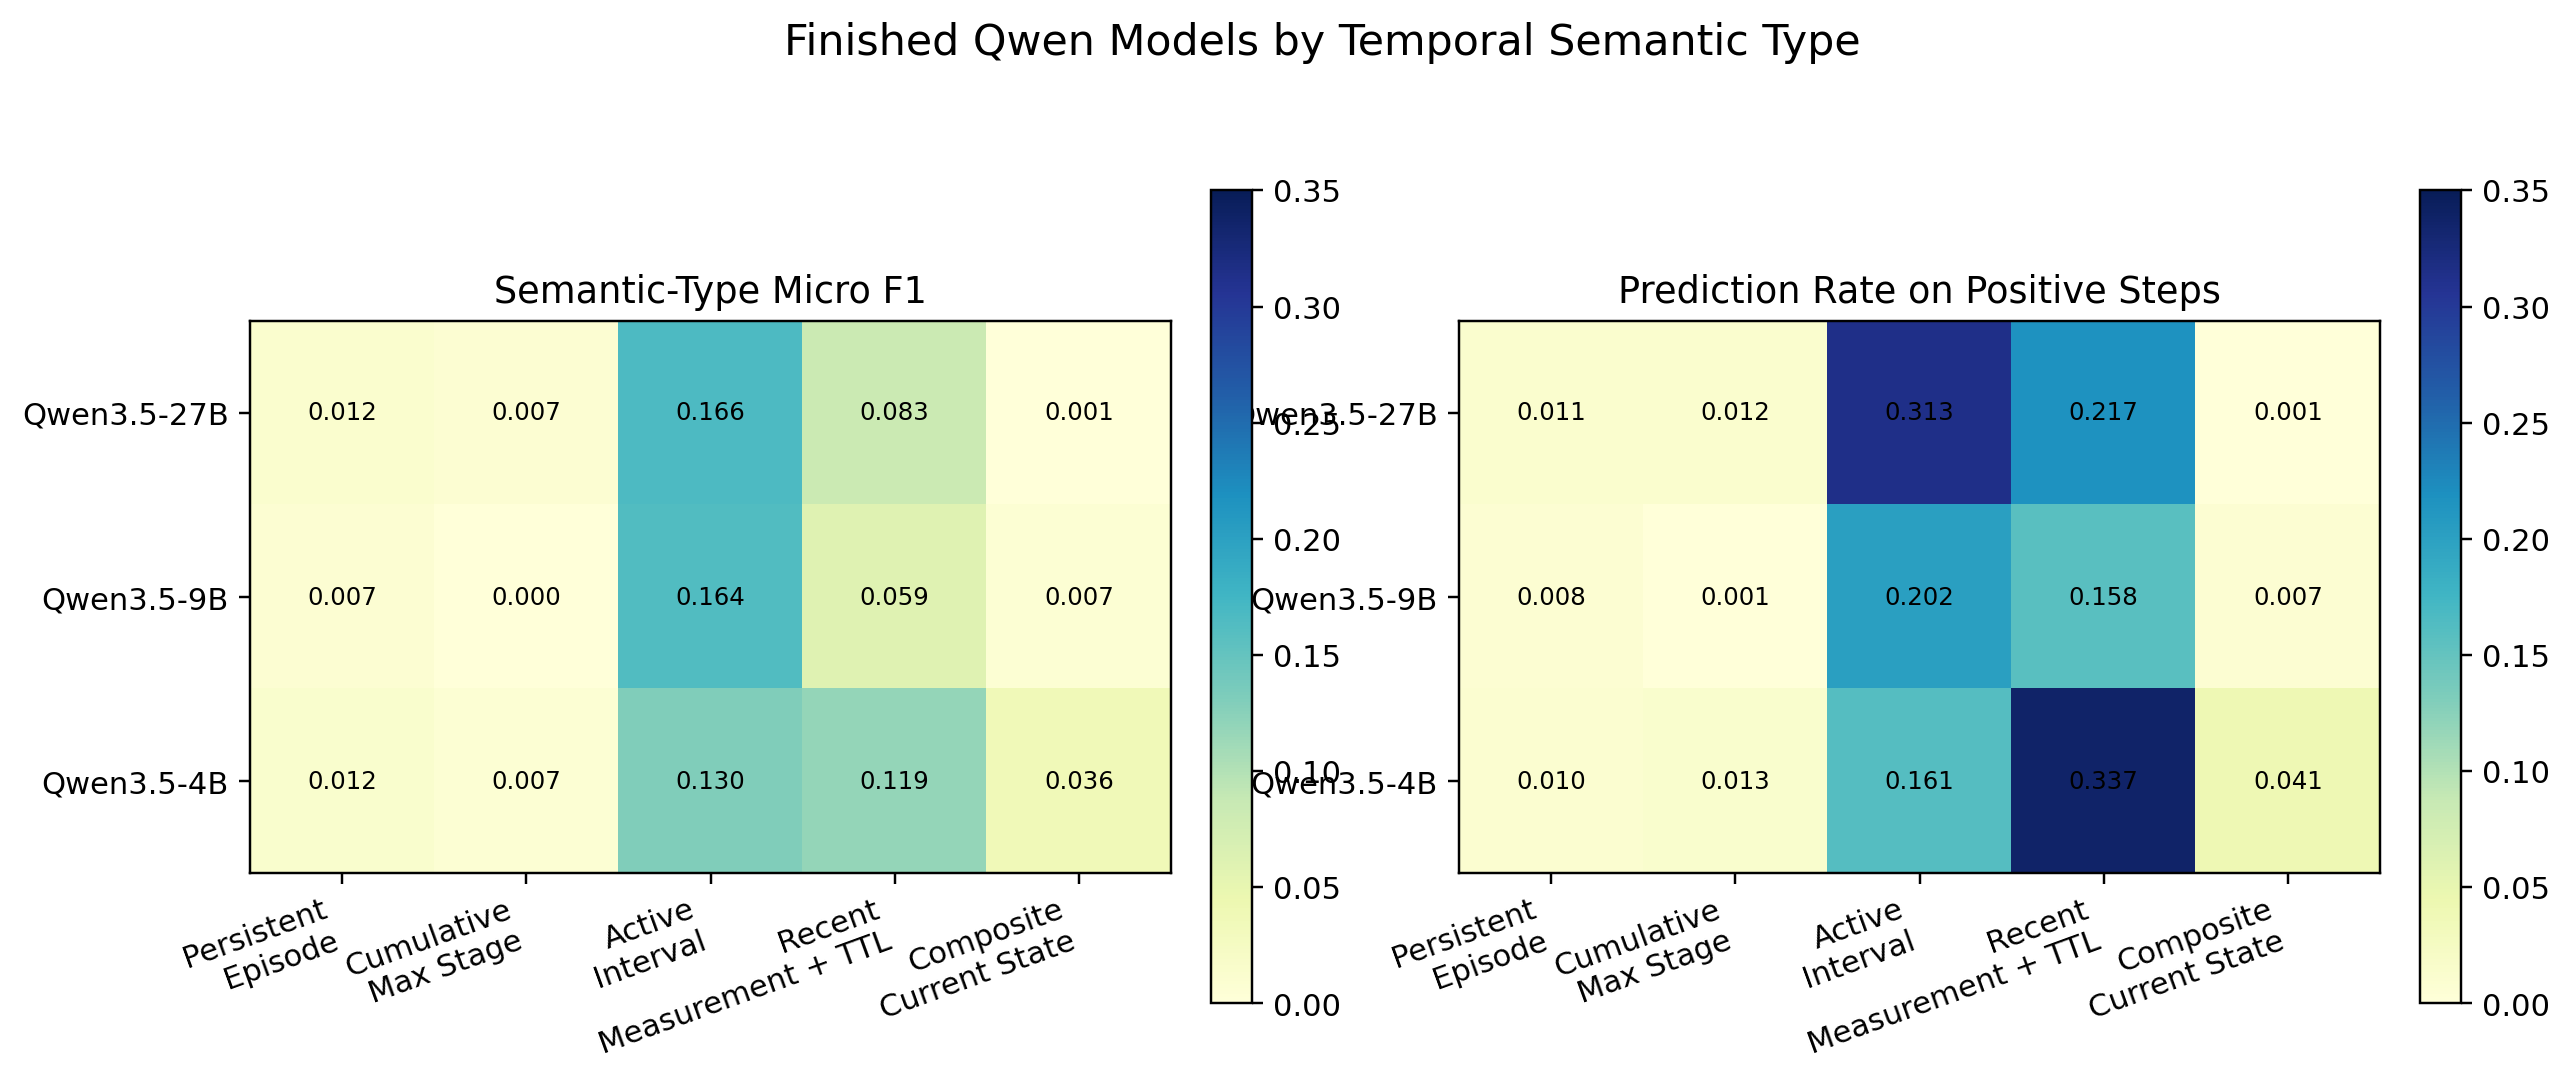
\includegraphics[width=0.84\textwidth]{figures/qwen_benchmark2k_semantic_heatmap.png}
\caption{Temporal-semantic analysis for the completed Qwen \texttt{benchmark\_2k} runs. The models are strongest on \texttt{active\_interval} states and weakest on \texttt{persistent\_episode}, \texttt{cumulative\_max\_stage}, and \texttt{composite\_current\_state}.}
\label{fig:qwen_semantics}
\end{figure*}

\subsection{Backend Matters: Zero-Shot vs Autoformalization}

The paired Qwen comparison on \texttt{benchmark\_100} shows that backend choice changes behavior in a structured, non-monotonic way. Autoformalization is not simply an easier version of the task, nor is zero-shot simply more faithful to the data. Instead, the two interfaces emphasize different temporal reasoning capabilities.

For the smaller Qwen models, autoformalization substantially improves coarse action calibration and alert-family recovery. Relative to zero-shot, the Qwen-family average on \texttt{benchmark\_100} rises from 0.2790 to 0.3682 in \texttt{global\_action\_accuracy}, from 0.2662 to 0.3487 in \texttt{priority\_accuracy}, and from 0.2335 to 0.2539 in \texttt{alerts\_macro\_f1}. Positive-only alert recovery improves even more sharply, from 0.0069 to 0.0326 macro F1 on average.

However, autoformalization does not uniformly improve suspect-family reasoning. \texttt{Qwen3.5-27B} performs better in zero-shot on suspect-family recovery (0.2063 versus 0.1942) and substantially better on positive-only suspect recovery (0.0510 versus 0.0165). It also misses fewer alerting trajectories in zero-shot (28 versus 53). Semantic analysis explains why: zero-shot \texttt{Qwen3.5-27B} preserves more \texttt{persistent\_episode}, \texttt{cumulative\_max\_stage}, and \texttt{composite\_current\_state} structure, whereas autoformalization helps mainly on \texttt{active\_interval} and, more modestly, \texttt{recent\_measurement + TTL}.

\begin{table*}[t]
\centering
\caption{Paired \texttt{benchmark\_100} comparison for the Qwen family across zero-shot raw-table access and autoformalization. Backend choice changes both accuracy and failure mode.}
\label{tab:qwen_backend_pair}
\resizebox{\textwidth}{!}{%
\begin{tabular}{llrrrrrrrr}
\toprule
Model & Mode & Suspect F1 & Alert F1 & Pos. Suspect F1 & Pos. Alert F1 & Global Action & Priority & First-alert MAE (h) & Missed alerts \\
\midrule
\texttt{Qwen3.5-27B} & autoformalization & 0.1942 & 0.2425 & 0.0165 & 0.0165 & 0.3869 & 0.3777 & 12.6829 & 53 \\
\texttt{Qwen3.5-27B} & zero-shot         & 0.2063 & 0.2195 & 0.0510 & 0.0176 & 0.3177 & 0.3108 & 12.0606 & 28 \\
\texttt{Qwen3.5-9B}  & autoformalization & 0.1856 & 0.2549 & 0.0050 & 0.0278 & 0.3531 & 0.3231 & 18.8148 & 67 \\
\texttt{Qwen3.5-9B}  & zero-shot         & 0.1847 & 0.2408 & 0.0019 & 0.0010 & 0.2492 & 0.2408 & 20.0000 & 83 \\
\texttt{Qwen3.5-4B}  & autoformalization & 0.1854 & 0.2643 & 0.0236 & 0.0534 & 0.3646 & 0.3454 & 11.2632 & 56 \\
\texttt{Qwen3.5-4B}  & zero-shot         & 0.1830 & 0.2401 & 0.0037 & 0.0021 & 0.2700 & 0.2469 & 11.5200 & 69 \\
\bottomrule
\end{tabular}%
}
\end{table*}

\begin{figure*}[t]
\centering
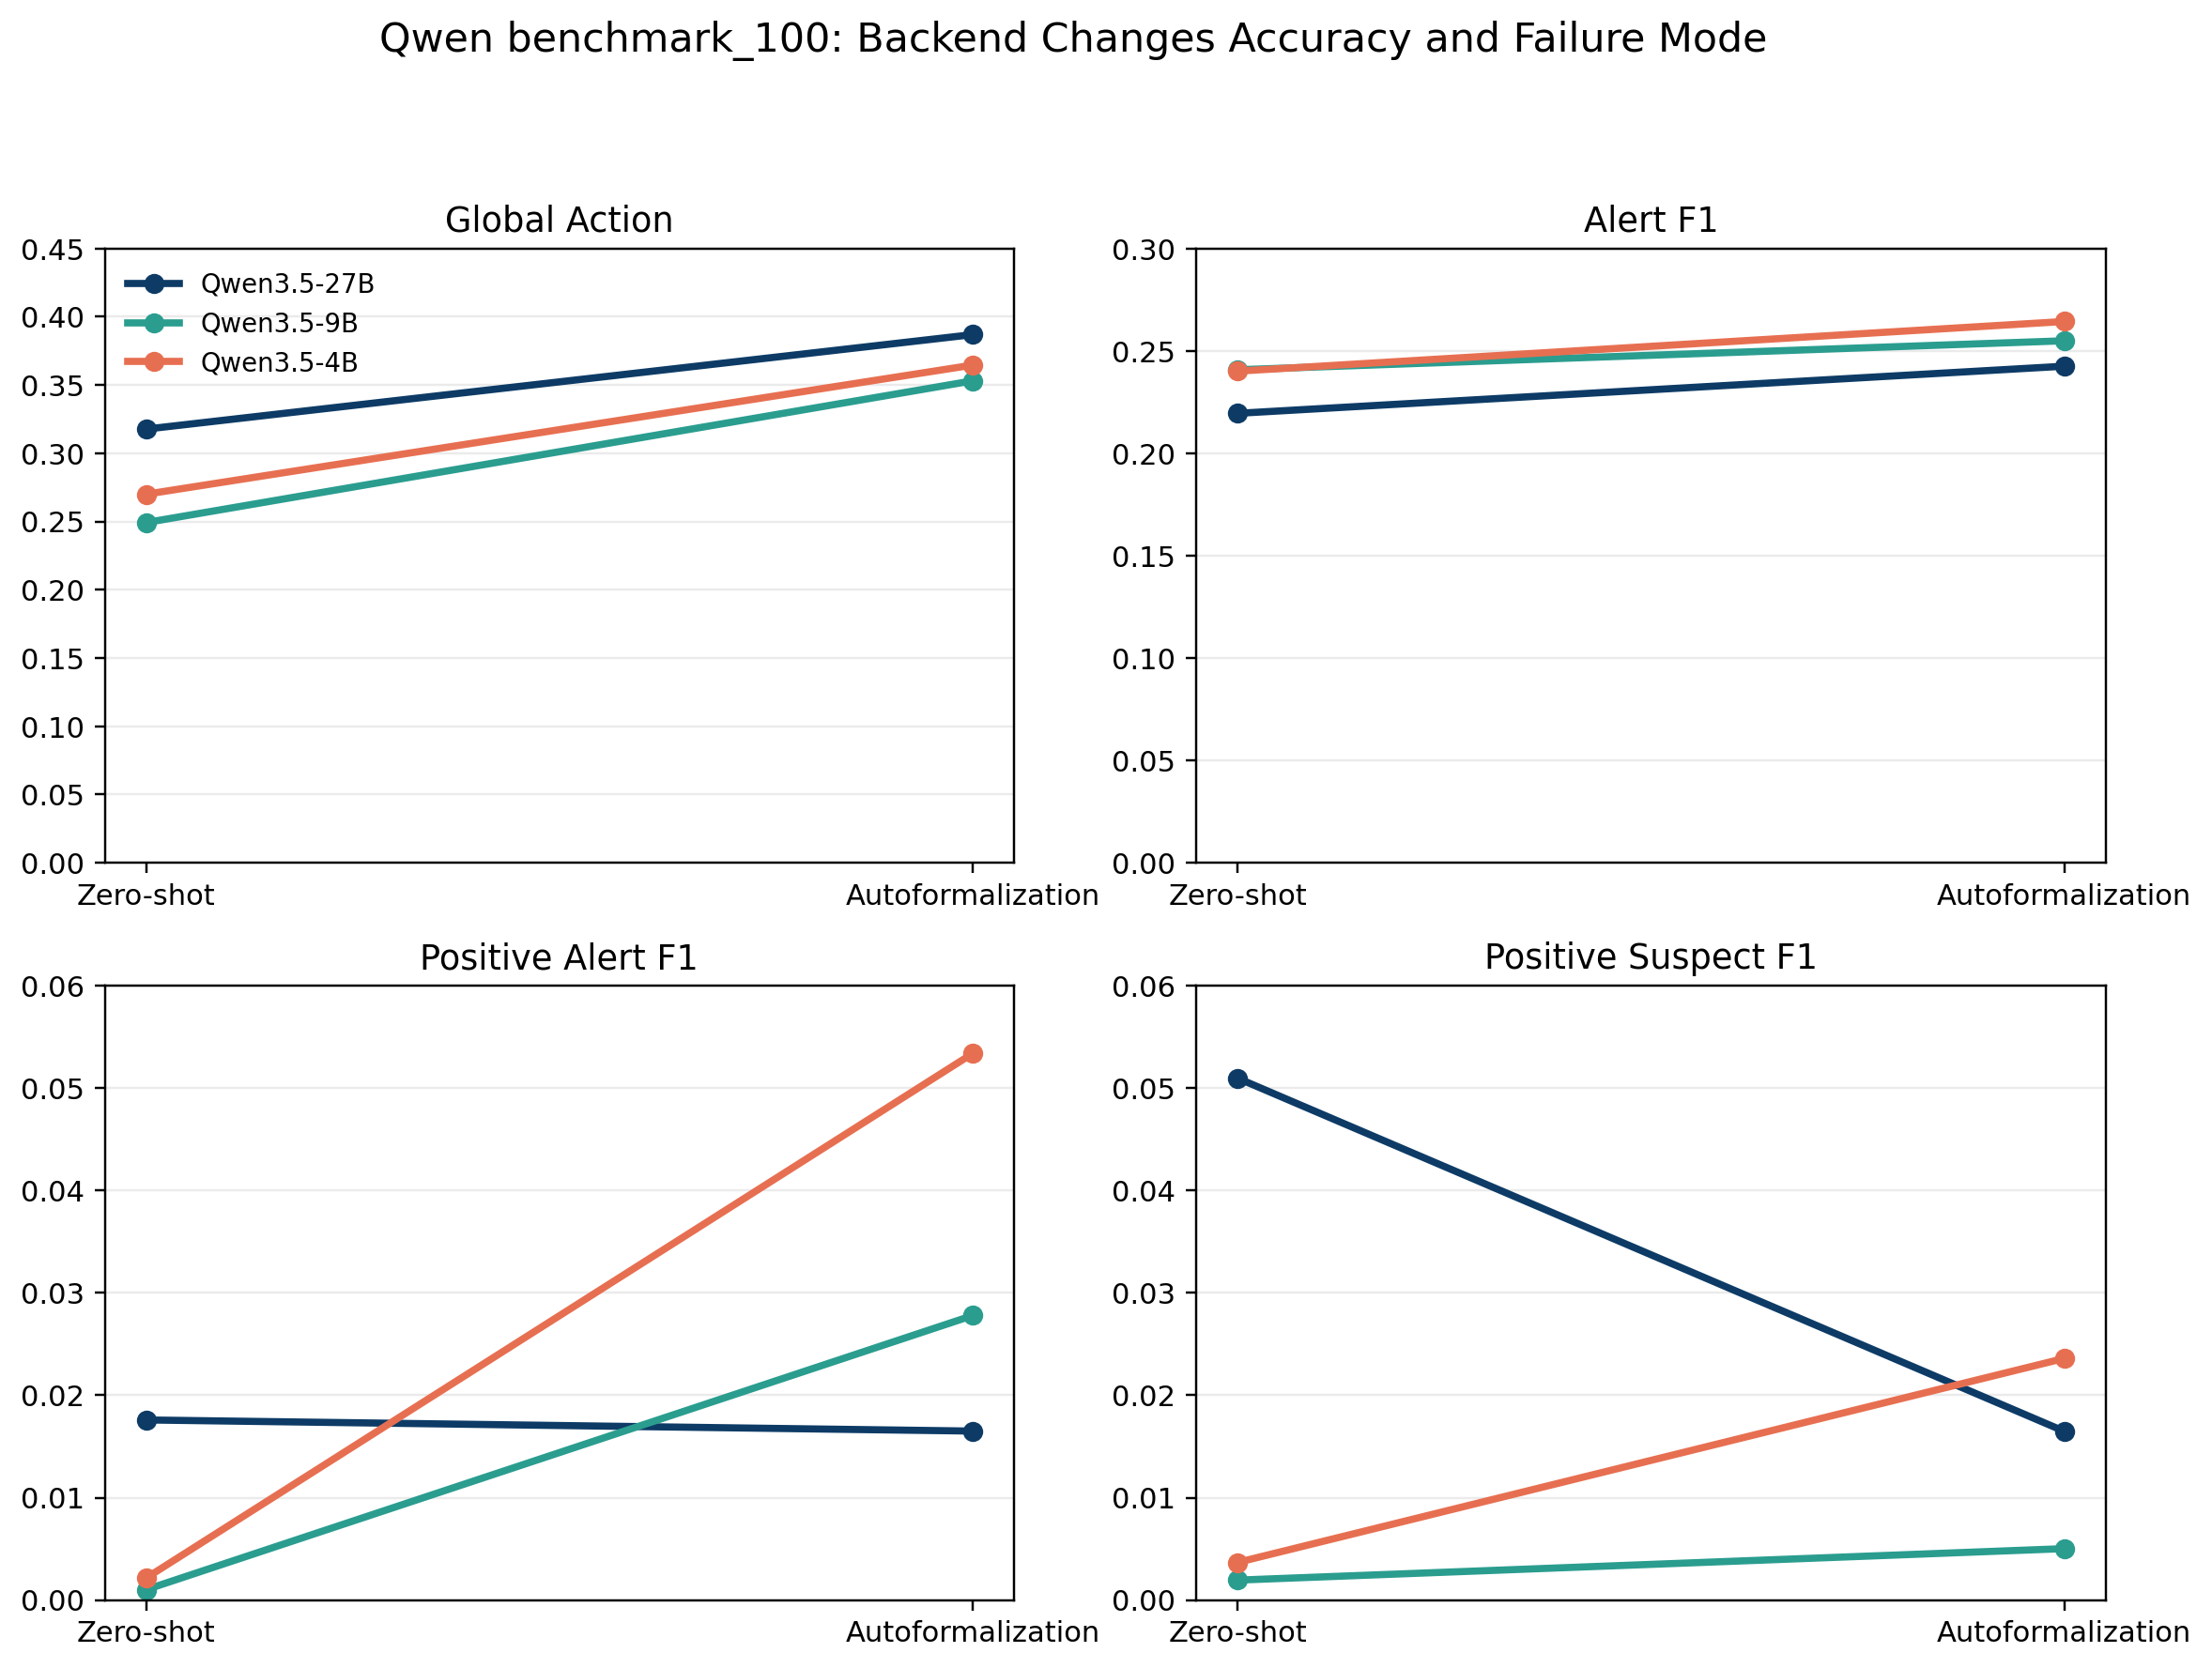
\includegraphics[width=0.82\textwidth]{figures/qwen_benchmark100_backend_comparison.png}
\caption{Paired Qwen comparison on \texttt{benchmark\_100}. Autoformalization generally improves action calibration and alert-family recovery for the smaller models, while zero-shot preserves stronger positive-only suspect recovery for \texttt{Qwen3.5-27B}.}
\label{fig:qwen_backend_compare}
\end{figure*}

\subsection{Open-Weight vs Closed-Source Models}

The open-weight versus closed-source conclusion depends on which backend is being evaluated.

In zero-shot raw-table \texttt{benchmark\_100}, the closed-source models are clearly stronger. Averaged across \texttt{GPT-5.4}, \texttt{Claude Sonnet 4.6}, and \texttt{Gemini 3.1 Pro Preview}, the closed-source group achieves 0.3595 \texttt{suspected\_conditions\_macro\_f1}, 0.4190 \texttt{alerts\_macro\_f1}, 5.22h first-alert mean absolute error, and 14.3 missed-alert trajectories. The corresponding open-weight averages are 0.2057, 0.2361, 12.84h, and 41.2. This is a large and consistent gap.

Within the closed-source zero-shot group, the ranking is itself meaningful. \texttt{Gemini} is best on suspect-family recovery and exact suspect-set matching, while \texttt{Claude} is best on alert-family recovery and timing, albeit with the most false-early alerts. \texttt{GPT-5.4} is clearly weaker than Claude and Gemini on the core structured-state metrics, but still stronger than the open-weight zero-shot models.

By contrast, the autoformalized setting does not yet permit a fair open-weight versus closed-source leaderboard claim. The only reliable completed \texttt{benchmark\_2k} evidence comes from open-weight models, because the autoformalized closed-source runs are incomplete and tool-error-heavy. Thus, the correct claim is backend-specific: closed-source models dominate the short raw-table pilot, while open-weight models currently provide the only completed evidence on the full autoformalized benchmark.

The cost profile of the open-weight zero-shot runs also helps explain some of this spread. After reconstructing the prompt stack from the saved zero-shot prompt template and per-step tool traces, the dominant cost source is not the tool outputs themselves but the repeated instruction scaffold plus checkpoint payload that must be re-sent on every model turn. Tool-output context is still substantial, especially for the larger open-weight models, accounting for roughly 13\% to 18\% of prompt-side cost. \texttt{Qwen3.5-27B} is the most expensive overall because it combines a large fixed prompt burden with high completion cost, while \texttt{gemma-4-31B-it} spends heavily on prompt-side interaction context but produces very few completion tokens. This suggests that some open-weight zero-shot failures are not simply low-effort shortcuts; several models incur heavy retrieval and control-flow cost without converting that interaction into stronger structured-state recovery.

\begin{table*}[t]
\centering
\caption{Completed zero-shot raw-table \texttt{benchmark\_100} comparison across open-weight and closed-source models. These results show a clear short-pilot advantage for closed-source systems, but do not replace the need for completed long-run evaluation.}
\label{tab:zeroshot_open_closed}
\resizebox{\textwidth}{!}{%
\begin{tabular}{llrrrrrr}
\toprule
Model & Family & Suspect F1 & Alert F1 & Suspect Exact & Alert Exact & First-alert MAE (h) & Missed alerts \\
\midrule
\texttt{Gemini/gemini-3.1-pro-preview} & closed-source & 0.4393 & 0.4636 & 0.2531 & 0.2423 & 4.6047 & 8 \\
\texttt{Claude/claude-sonnet-4-6} & closed-source & 0.3830 & 0.4722 & 0.1808 & 0.2338 & 3.9535 & 8 \\
\texttt{GPT/gpt-5.4} & closed-source & 0.2561 & 0.3212 & 0.1862 & 0.2192 & 7.1045 & 27 \\
\texttt{gpt-oss-120b} & open-weight & 0.2564 & 0.2167 & 0.1715 & 0.1831 & 11.3333 & 4 \\
\texttt{Qwen3.5-27B} & open-weight & 0.2063 & 0.2195 & 0.1800 & 0.2062 & 12.0606 & 28 \\
\texttt{gemma-4-31B-it} & open-weight & 0.1982 & 0.2632 & 0.1646 & 0.2046 & 9.2778 & 22 \\
\texttt{Qwen3.5-9B} & open-weight & 0.1847 & 0.2408 & 0.1831 & 0.2408 & 20.0000 & 83 \\
\texttt{Qwen3.5-4B} & open-weight & 0.1830 & 0.2401 & 0.1815 & 0.2385 & 11.5200 & 69 \\
\bottomrule
\end{tabular}%
}
\end{table*}

\begin{figure*}[t]
\centering
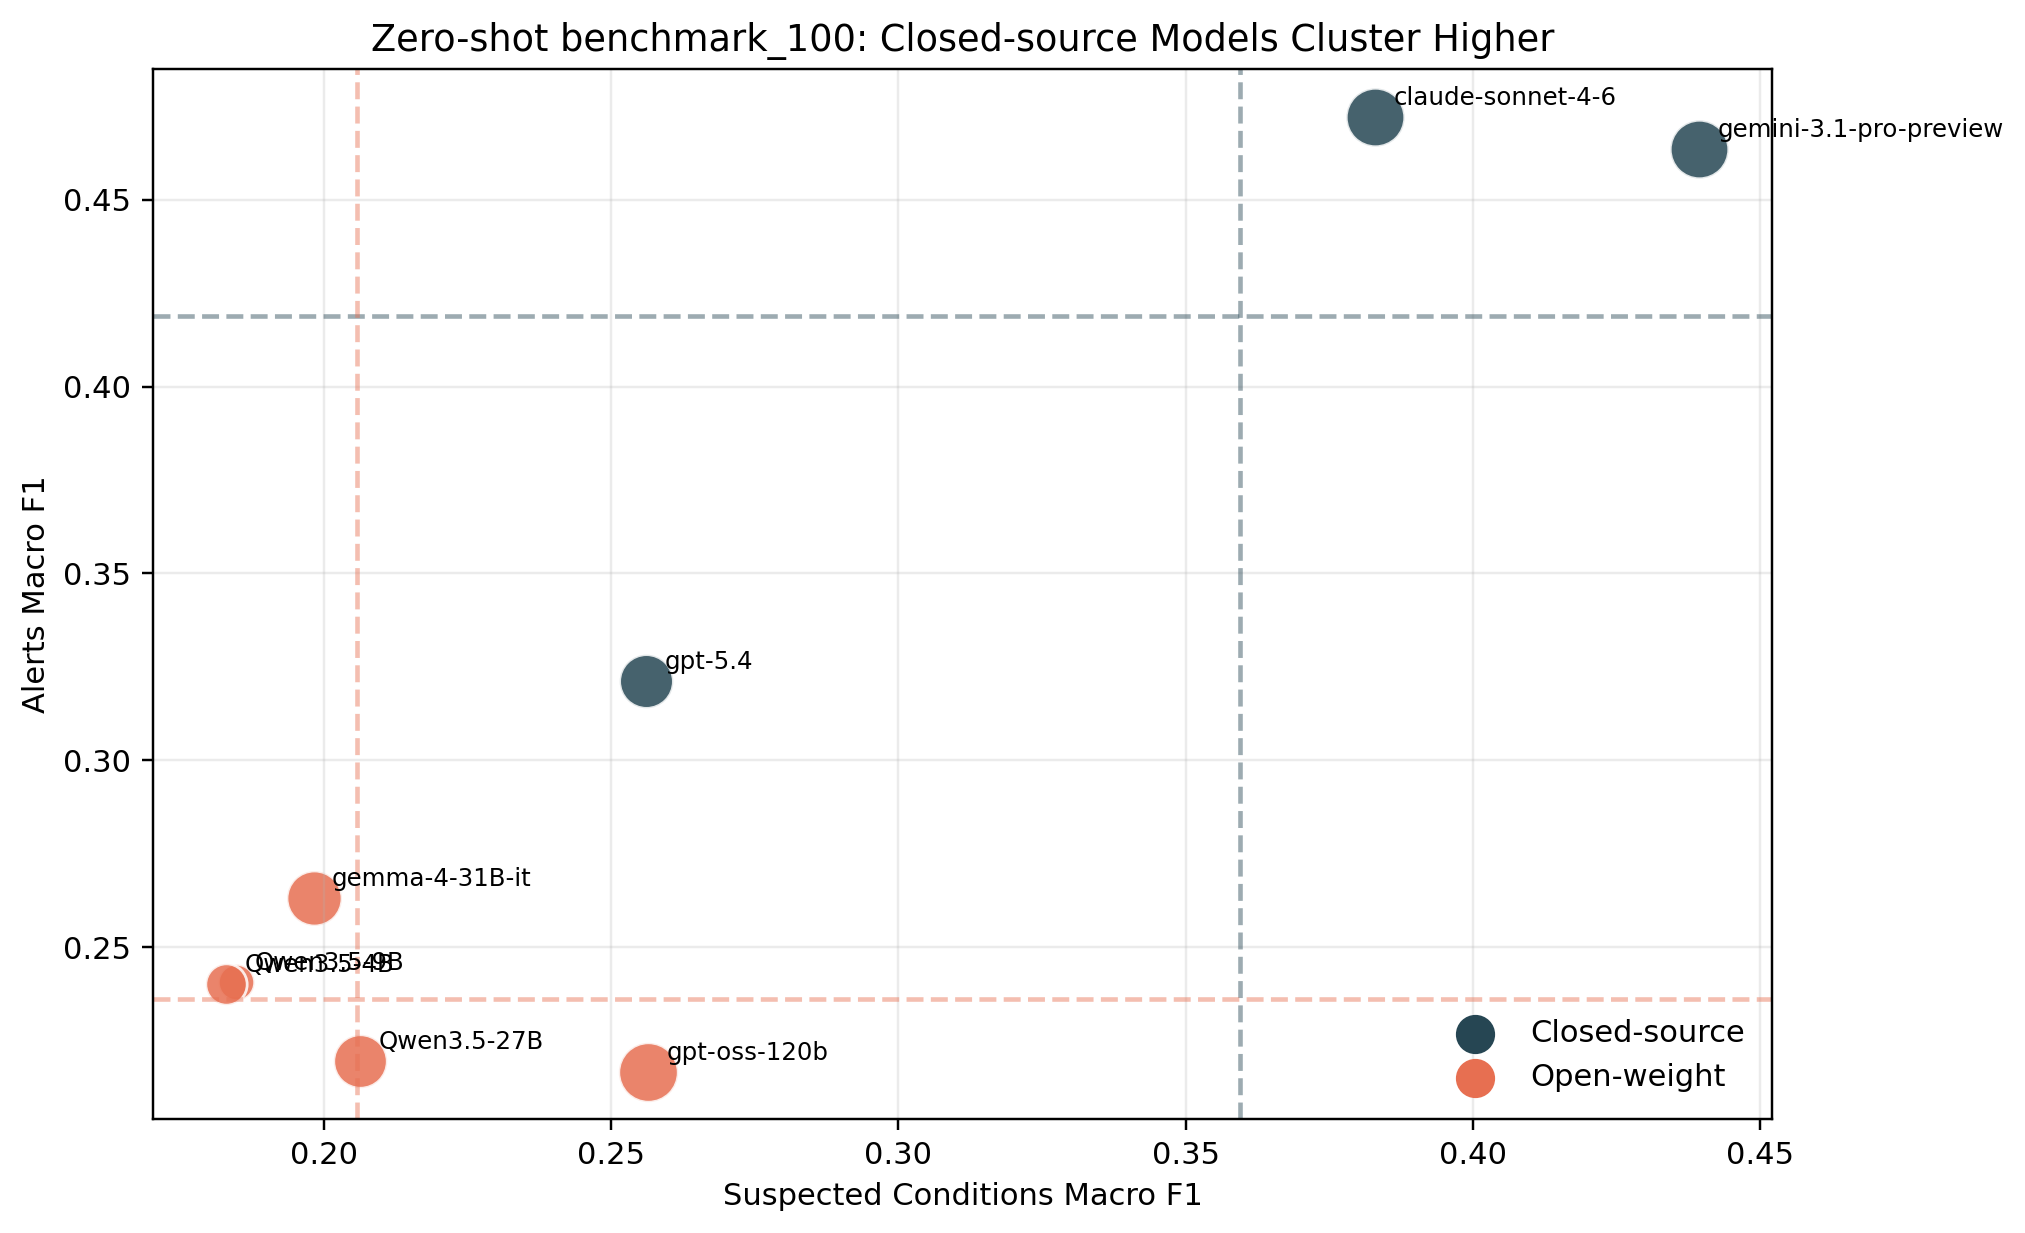
\includegraphics[width=0.76\textwidth]{figures/zeroshot_benchmark100_open_vs_closed.png}
\caption{Completed zero-shot raw-table \texttt{benchmark\_100} comparison. Closed-source models cluster in the upper-right, indicating stronger joint suspect- and alert-family recovery than the open-weight zero-shot models.}
\label{fig:zeroshot_open_closed}
\end{figure*}

\begin{figure*}[t]
\centering
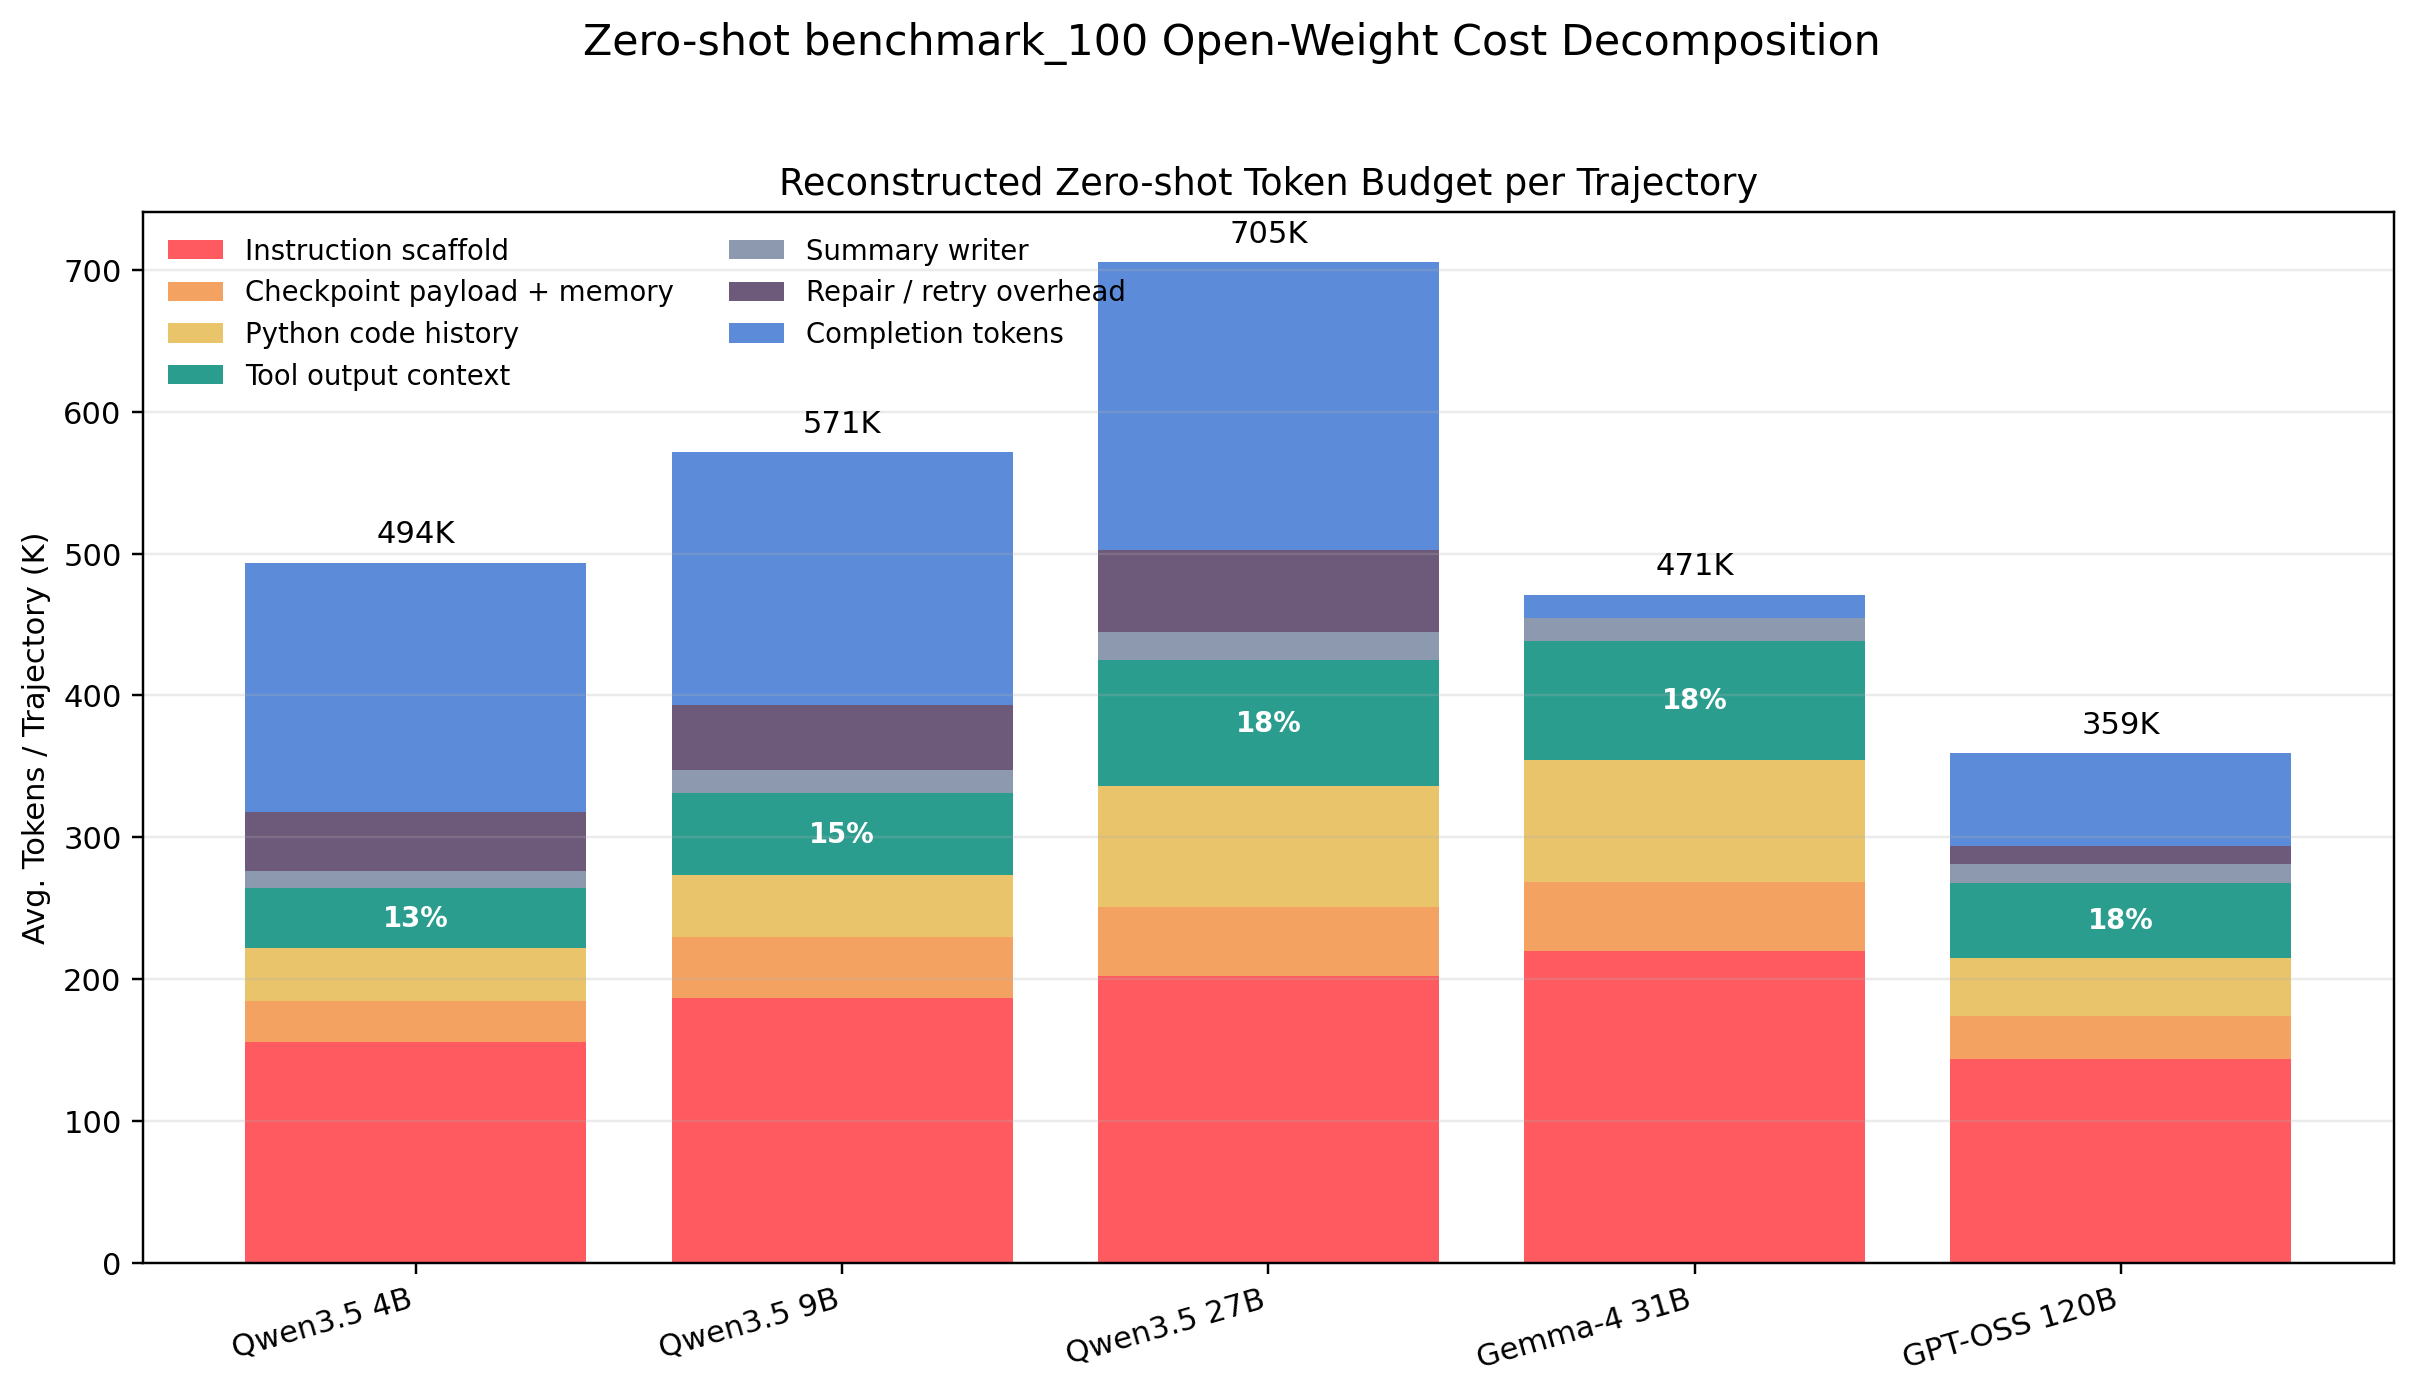
\includegraphics[width=0.92\textwidth]{figures/zeroshot_benchmark100_open_weight_cost_breakdown.png}
\caption{Open-weight zero-shot cost decomposition on \texttt{benchmark\_100}. Each stacked bar reconstructs average tokens per trajectory into fixed instruction scaffold, checkpoint payload plus rolling memory, accumulated Python code history, accumulated tool-output context, summary-writer overhead, estimated repair/retry overhead, and measured completion tokens. The prompt-side split is reconstructed from the saved backend prompt template and per-step tool traces, while the completion segment is directly measured.}
\label{fig:zeroshot_open_weight_cost}
\end{figure*}

\subsection{Failure Modes}

The combined results expose two broad failure classes: conceptual longitudinal reasoning failures and interface-mediated infrastructure failures.

The most important conceptual failure is conservative collapse. Many open-weight models, especially in zero-shot, drift toward near-always \texttt{continue\_monitoring} behavior. On raw-table \texttt{benchmark\_100}, \texttt{Qwen3.5-9B} predicts \texttt{continue\_monitoring} on 98.92\% of steps and \texttt{Qwen3.5-4B} on 96.54\%. The partial zero-shot \texttt{benchmark\_2k} \texttt{Qwen3.5-4B} run is even more extreme at 98.15\%. This collapse explains why overall exact-match can still look superficially moderate while positive-only alert recovery is near zero.

The second conceptual failure is semantic selectivity. Even when models avoid complete conservative collapse, they tend to recover only the easiest temporal semantics. The completed Qwen \texttt{benchmark\_2k} runs are strongest on \texttt{active\_interval}, weaker on \texttt{recent\_measurement + TTL}, and extremely weak on \texttt{persistent\_episode}, \texttt{cumulative\_max\_stage}, and \texttt{composite\_current\_state}. This indicates that maintaining persistent and cumulative state across checkpoints is harder than detecting currently visible support or measurement states.

The main interface-mediated failure lies in tool reliability and callable discoverability. In the autoformalized \texttt{session\_tools} setting, repeated failures cluster around a small set of helpers, including blood-gas, vasoactive, KDIGO, and GCS-related functions. These issues are especially severe in the autoformalized closed-source pilots, which makes those runs unsuitable for definitive comparison. At the same time, the backend contrast suggests that interface design genuinely changes the reasoning profile, so the observed differences cannot be dismissed as pure infrastructure noise.

Overall, the results support three main conclusions. First, longitudinal structured-state tracking, rather than coarse escalation detection, is the core bottleneck of the benchmark. Second, backend choice materially changes which temporal semantics models can recover, so zero-shot raw-table reasoning and autoformalization should be treated as substantively different evaluation conditions. Third, while frontier closed-source models are strongest in the short raw-table pilot, the only reliable completed evidence on the full \texttt{benchmark\_2k} benchmark currently comes from open-weight models, and even the best completed run remains far from robust patient-level surveillance-state tracking.
